% !TEX root = ../../ozan_sener_thesis.tex

\section{Overview of rCRF}
\label{overview}
\begin{figure}[t]
\centering
  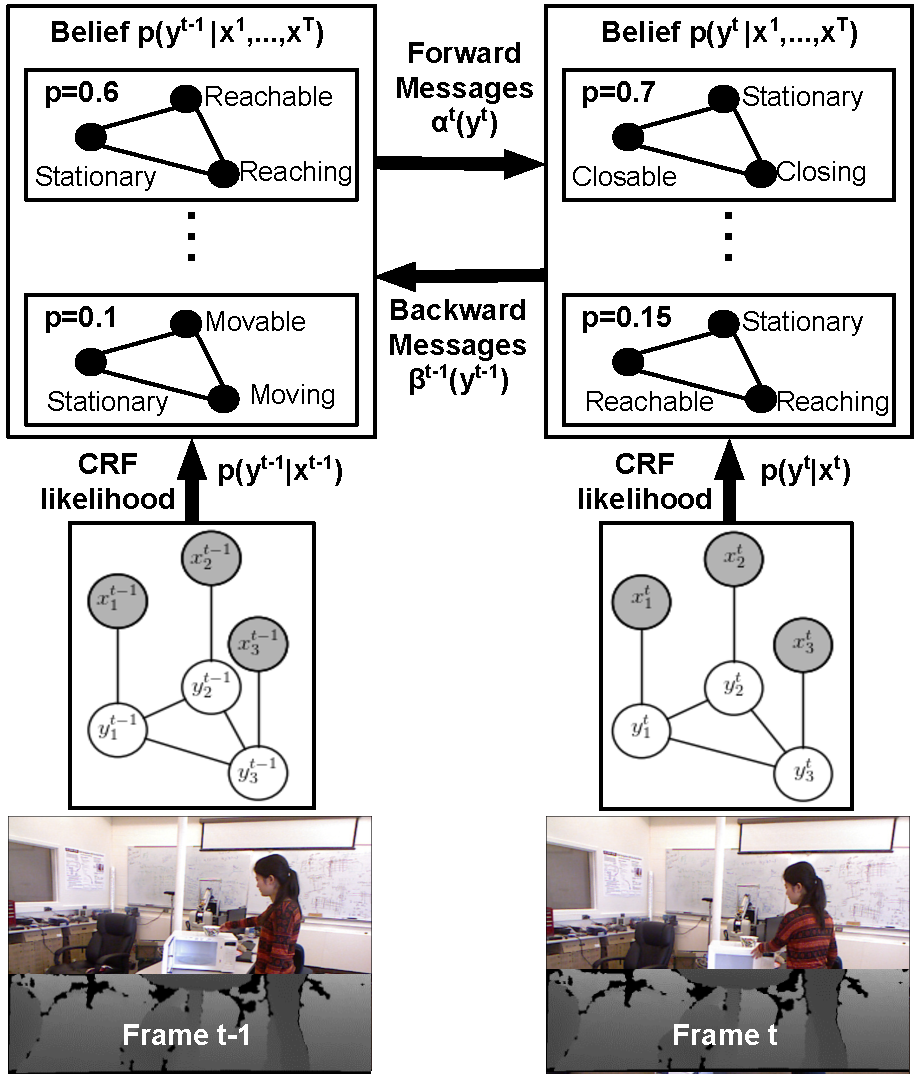
\includegraphics[width=0.7\textwidth]{systemflow}
  \caption{{\bf Computing the full belief by using rCRF.} Each iteration of the recursive estimation algorithm includes computing forward and backward messages, $\alpha^t(\mathbf{y}^t)$ and $\beta^{t-1}(\mathbf{y}^{t-1})$, by using the current samples and computing the belief $p(\mathbf{y}^t|\mathbf{x}^1,\ldots,\mathbf{x}^T)$ with the computed messages. Then, we re-compute the messages and re-sample the belief until the belief converges. \emph{Here, we only have two objects as  $\mathbf{y}^t=(\mathbf{O}^t_1,\mathbf{O}^t_2,\mathbf{A}^t)$ and $\mathbf{x}^t=(\mathbf{L}^t_1,\mathbf{L}^t_2,\mathbf{H}^t)$ }}
  \label{system}
\end{figure}
%Toy Example
In this section, we summarize our method and explain how we estimate the full belief over the activities and object affordances. Moreover, we also give an illustrative example of the rCRF with a toy scene consisting of two objects (a microwave and a bowl) and a human in Figure~\ref{system}.

%CRF
Reasoning about activities requires not only identifying the objects but also interpreting object-object relations and human-object relations. Indeed, we capture such rich information via CRF. As shown in the Figure~\ref{system}, each object and a human corresponds to a node in the graph on which we define the CRF. As a hidden variable, we are interested in object affordances such as \emph{openable, graspable, movable, etc.}, and the activity human is performing such as \emph{moving, opening, grasping, etc.}. We define the affordances as the actions that can be performed on/with the object~\cite{gibson1979}. We denote the affordance variables at time $t$ as $\mathbf{O}^t_1, \ldots, \mathbf{O}^t_N$ for $N$ objects and the activity variable as $\mathbf{A}^t$. Since they are not directly observed, we estimate them by using partial observations. We are using the 3D positions of the objects $\mathbf{L}^t_1,\ldots,\mathbf{L}^t_N$ and the human pose $\mathbf{H}^t$ as observations. %Human pose corresponds to the 3D position of the joints of the human in the scene.
The input video is temporally over-segmented prior to the application of the belief estimation, and the time instant $t$ represent the $t^{th}$ segment of the video. We explain the features and the potential functions we use while defining the CRF in Section~\ref{rgbd}.

In addition to the spatial relations between objects and humans, we are also interested in their temporal evolution. In general, the problem of estimating a belief over set of hidden variables using the entire video corresponds to a Bayesian smoothing problem. Formally, we are interested in estimating states \mbox{$\mathbf{y}^t=(\mathbf{O}_1^t,\ldots,\mathbf{O}_N^t,\mathbf{A}^t)$} given set of observations \mbox{$\mathbf{x}^t=(\mathbf{L}_1^t,\ldots,\mathbf{L}_N^t,\mathbf{H}^t)$}. We estimate the states through successive application of the recursive Bayesian updates. In order to tractably compute the Bayesian updates, we introduce two approximations in Section~\ref{theory}. First, we compute the set of all plausible future states by using structured-diversity. Second, we use Jensen inequality in order to convert the discriminative likelihood into a generative one. After the introduction of these two machineries, we follow the recursive Bayesian estimation framework. As shown in Figure~\ref{system}, we first compute the Bayesian updates through the forward and backward messages, $\alpha^t(\mathbf{y}^t)$ and $\beta^{t}(\mathbf{y}^{t})$. We then compute the posterior belief $p(\mathbf{y}^t|\mathbf{x}^1,\ldots,\mathbf{x}^T)$ by using the computed messages and the CRF-likelihood \emph{$p(\mathbf{y}^t|\mathbf{x}^t)$}. As a final step of the iteration, we represent the belief via diverse samples of the posterior belief. Since the belief is recursively defined, we re-compute the messages and re-sample the belief until it converges.

%We denote the observation as $\bf{x^t}$ and the hidden state as $\bf{y^t}$ for clarity. After defining the rCRF and developing the algorithm in Section~\ref{theory}, we return to the problem of activity analysis and its notation in Section~\ref{rgbd}.
